%% -*- coding: utf-8 -*-
\documentclass[12pt,a4paper]{scrartcl} 
\usepackage[utf8]{inputenc}
\usepackage[english,russian]{babel}
\usepackage{indentfirst}
\usepackage{misccorr}
\usepackage{graphicx}
\usepackage{amsmath}
\usepackage{xcolor} 
\usepackage{listings} 

% Настройка стиля для C++
\lstset{
	language=C++,
	inputencoding=utf8,
	extendedchars=true,
	basicstyle=\small\ttfamily,
	keywordstyle=\bfseries\color{blue},
	commentstyle=\itshape\color{gray},
	stringstyle=\color{red},
	showstringspaces=false,
	breaklines=true,
	frame=single,
	tabsize=2
}


\begin{document}
	\begin{center}
		\large{\textbf{Отчет по лабораторной работе}} \\
		\large{\textbf{Тема: «Реализация семантической сети»}}
	\end{center}
	
	\section{Введение}
	\label{sec:intro}
	
	\subsection{Текстовая формулировка задачи}
	\label{sec:intro:task}
	Целью работы является разработка программного комплекса на языке C++, реализующего модель семантической сети. Программа должна обеспечивать создание структуры сети путем парсинга данных из внешнего файла формата JSON. В памяти объекты и связи между ними должны быть представлены с помощью соответствующих структур данных. Программный интерфейс должен предоставлять базовые функции для взаимодействия с сетью: вывод полной иерархической структуры, а также выполнение поисковых запросов для нахождения объектов и связей.
	
	\subsection{Пример кода, решающего задачу}
	\label{sec:intro:code}
	Пример использования основных функций библиотеки представлен в функции `main`. Данный код инициализирует семантическую сеть из файла, выводит ее полную структуру, а затем выполняет два типа поиска: поиск объекта по отношению и поиск отношения по имени целевого объекта.
	
	\begin{lstlisting}[caption={Пример основной логики приложения}]
		int main() {
			setlocale(LC_ALL, "Russian");
			
			if (gSemantic.Create())
			{
				for (int i = 0; i < gSemantic.StaticObjects.size(); i++)
				{
					gSemantic.PrintObject(gSemantic.StaticObjects.at(i));
					std::cout << std::endl << "---------------------------" << std::endl;;
				}
				
				auto Founded = gSemantic.FindObjectByRelation(gSemantic.GetObjectByName("Petya"), "has_a");
				
				if (!Founded.empty())
				{
					for (int i = 0; i < Founded.size(); i++)
					{
						std::cout << "Object by relation: " << Founded.at(i)->Name << std::endl;
					}
				}
				
				std::string FoundedRelation = gSemantic.FindRelationByObject(gSemantic.GetObjectByName("Petya"), "hairs");
				
				std::cout << "Relation by object: " << FoundedRelation.c_str() << std::endl;
				
				gSemantic.Destroy();
			}
			else
			std::cout << "Parse error" << std::endl;
			
			system("pause");
			return 0;
		};
	\end{lstlisting}
	
	\subsection{Концептуальный граф и результат работы}
	\label{sec:intro:graph}
	На рисунке~\ref{fig:graph} представлена концептуальная схема небольшой части семантической сети. На рисунке~\ref{fig:screenshot} показан результат работы программы, демонстрирующий вывод данных.
	
	\begin{figure}[h!]
		\centering
		\fbox{\parbox{0.8\textwidth}{
				\centering
				\vspace{1cm}
				\textbf{[Концептуальная схема графа]} \\
				\vspace{0.5cm}
				Узел: "Petya" \\
				\textit{Связь: "has\_a"} $\rightarrow$ Узел: "hairs" \\
				\textit{Связь: "has\_a"} $\rightarrow$ Узел: "head" \\
				\vspace{0.2cm}
				Узел: "hairs" \\
				\textit{Связь: "is\_a"} $\rightarrow$ Узел: "object" \\
				\vspace{0.2cm}
				Узел: "head" \\
				\textit{Связь: "part\_of"} $\rightarrow$ Узел: "body" \\
				\vspace{1cm}
		}}
		\caption{Концептуальная схема части семантической сети}\label{fig:graph}
	\end{figure}
	
	\begin{figure}[h!]
		\centering
		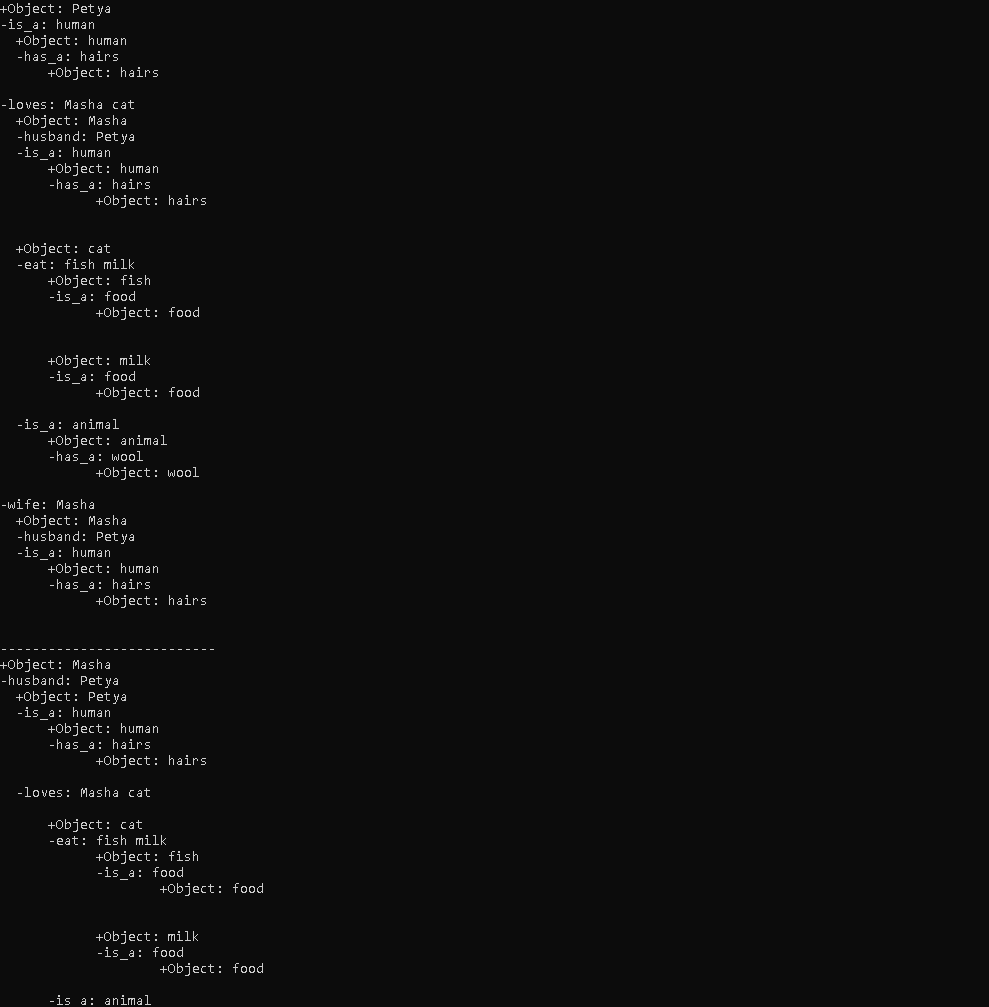
\includegraphics[width=0.9\textwidth]{Output.png}
		\caption{Пример вывода программы}\label{fig:screenshot}
	\end{figure}
	
	
	\section{Ход работы}
	\label{sec:exp}
	
	\subsection{Структуры данных}
	\label{sec:exp:struct}
	В основе реализации лежит структура `cObject`, которая представляет узел семантической сети. Каждый объект имеет имя (`std::string Name`) и набор отношений (`Relations`), реализованный через `std::map`. Ключом в `map` является имя отношения (например, "is\_a", "has\_a"), а значением — вектор указателей (`std::vector<pObject>`) на объекты, с которыми установлена данная связь. Это позволяет одному объекту иметь множество связей разных типов с разными объектами.
	
	\begin{lstlisting}[caption={Определение структуры объекта}]
		typedef struct cObject {
			std::string Name;
			std::map<std::string, std::vector<pObject>> Relations;
		} *pObject;
	\end{lstlisting}
	
	\subsection{Основные компоненты программы}
	\label{sec:exp:components}
	Программа состоит из нескольких ключевых компонентов: парсера JSON и класса для управления семантической сетью.
	
	\subsubsection{Парсер JSON}
	Отвечает за чтение и интерпретацию файла `Objects.json`. Он последовательно создает все объекты, а затем, на втором проходе, устанавливает связи между ними, используя ранее созданные экземпляры. Для работы с JSON используется библиотека `nlohmann/json`.
	
	\begin{lstlisting}[caption={Функция парсинга JSON}]
		bool cParser::ParseJson(std::vector<pObject> &Objects, std::string Path)
		{
			std::ifstream InputFile(Path);
			if (!InputFile.is_open()) {
				return false;
			}
			
			json Data;
			InputFile >> Data;
			
			for (const auto& NodeJson : Data["objects"]) {
				Objects.push_back(gSemantic.AddObject(NodeJson["name"]));
			}
			
			for (const auto& RelationJson : Data["relations"]) {
				std::string Relation = RelationJson["relation"];
				pObject Source = gSemantic.GetObjectByName(RelationJson["source"], Objects);
				pObject Target = gSemantic.GetObjectByName(RelationJson["target"], Objects);
				if (Source && Target)
				gSemantic.AddRelation(Source, Target, Relation);
			}
			
			return true;
		}
	\end{lstlisting}
	
	\subsubsection{Класс семантической сети и рекурсивный обход графа}
	Класс `cSemantic` инкапсулирует всю логику работы с сетью. Ключевые операции, такие как поиск и вывод, реализованы с помощью рекурсивного обхода графа.
	
	\paragraph{Вывод иерархии.} Метод `PrintObject` рекурсивно обходит связи объекта и выводит их с отступами для наглядного отображения иерархии. Глубина рекурсии отслеживается переменной `Cycles` для корректного форматирования.
	\begin{lstlisting}[caption={Рекурсивный вывод структуры сети}]
		void cSemantic::PrintObject(pObject Object, pObject EntryObject)
		{
			std::cout << Ladder(Cycles) << "+Object: " << Object->Name << std::endl;
			
			if(Object->Relations.empty())
			std::cout << std::endl;
			
			for (auto const& [RelationName, Objects] : Object->Relations)
			{
				std::cout << Ladder(Cycles) << "-" << RelationName << ": ";
				for (pObject FoundedObject : Objects) {
					std::cout << FoundedObject->Name << " ";
				}
				
				for (pObject FoundedObject : Objects)
				{
					if (EntryObject == FoundedObject)
					{
						std::cout << std::endl;
						continue;
					}
					
					if (FoundedObject)
					{
						Cycles++;
						std::cout << std::endl;
						PrintObject(FoundedObject, EntryObject ? EntryObject : Object);
					}
				}
			}
			
			if(Cycles > 0)
			Cycles--;
		}
	\end{lstlisting}
	
	\paragraph{Поиск по графу.} Рассмотрим механизм рекурсии на примере функции `FindObjectByRelation`. Функция принимает на вход текущий объект для проверки (`Object`), имя искомой связи (`Name`) и `EntryObject` — узел, из которого был совершен переход на текущий уровень рекурсии.
	
	Принцип работы следующий:
	\begin{enumerate}
		\item \textbf{Прямой поиск:} Функция проверяет, есть ли у текущего объекта `Object` связь с именем `Name`. Если есть, она найдена, и функция возвращает связанные с ней объекты.
		\item \textbf{Рекурсивный шаг:} Если прямой поиск не дал результатов, функция переходит к обходу в глубину. Она итерирует по всем связям текущего объекта.
		\item \textbf{Предотвращение зацикливания:} Перед тем как совершить рекурсивный вызов для связанного объекта (`FoundedObject`), происходит проверка `if (EntryObject == FoundedObject)`. Это необходимо, чтобы избежать бесконечного цикла в случае двунаправленных связей (например, A $\leftrightarrow$ B). Параметр `EntryObject` не позволяет функции вернуться в узел, из которого она только что пришла.
		\item \textbf{Вызов самой себя:} Если проверка на зацикливание пройдена, функция вызывает саму себя для связанного узла: `FindObjectByRelation(FoundedObject, Name, Object)`. Текущий объект `Object` передается как `EntryObject` для следующего уровня рекурсии.
	\end{enumerate}
	Такой подход позволяет обойти всю достижимую из начальной точки часть графа. Аналогичный механизм используется и в других поисковых методах класса.
	
	\begin{lstlisting}[caption={Рекурсивный поиск объекта по связи}]
		std::vector<pObject> cSemantic::FindObjectByRelation(pObject Object, std::string Name, pObject EntryObject)
		{
			std::vector<pObject> FoundedObjects;
			
			if (!Object || Name == "")
			return FoundedObjects;
			
			for (auto const& [RelationName, Objects] : Object->Relations)
			{
				if (RelationName == Name)
				{
					FoundedObjects = Objects;
				}
				else
				{
					for (pObject FoundedObject : Objects)
					{
						if (EntryObject == FoundedObject)
						{
							continue;
						}
						
						if (FoundedObject)
						{
							if (!EntryObject)
							FoundedObjects = FindObjectByRelation(FoundedObject, Name, Object);
							else
							FoundedObjects = FindObjectByRelation(FoundedObject, Name, EntryObject);
						}
					}
				}
			}
			
			return FoundedObjects;
		}
	\end{lstlisting}
	
	\section{Заключение}
	\label{sec:conclusion}
	В ходе выполнения работы была успешно реализована программная библиотека для создания и анализа семантической сети. Разработанные структуры данных и рекурсивные алгоритмы позволяют эффективно представлять и обрабатывать объекты и их связи, загруженные из внешнего JSON-файла. Функциональность вывода и поиска, продемонстрированная в приведенных примерах кода и на рисунке~\ref{fig:screenshot}, подтверждает корректность работы реализованной модели.
	
	\begin{thebibliography}{9}
		\bibitem{Knuth-2003}Кнут Д.Э. Всё про \TeX. \newblock --- Москва: Изд. Вильямс, 2003 г. 550~с.
		\bibitem{Lvovsky-2003}Львовский С.М. Набор и верстка в системе \LaTeX{}. \newblock --- 3-е издание, исправленное и дополненное, 2003 г.
		\bibitem{Voroncov-2005}Воронцов К.В. \LaTeX{} в примерах. 2005 г.
	\end{thebibliography}
	
\end{document}